\documentclass[tikz,border=5mm]{standalone}
\usepackage[T1]{fontenc}
\usepackage{lmodern}
\usepackage{amsmath,amssymb}
\usepackage{xcolor}
\usepackage{tikz}
\usetikzlibrary{arrows.meta,positioning,calc,fit,backgrounds,decorations.pathreplacing,shapes.geometric}
\tikzset{
  doc/.style = {rectangle, draw, rounded corners=2pt, minimum width=1.2cm, minimum height=0.6cm, fill=blue!10},
  sum/.style = {rectangle, draw, rounded corners=3pt, minimum width=2.35cm, minimum height=1.05cm, align=center, inner sep=3pt, fill=green!8},
  plus/.style = {circle, draw, minimum size=0.42cm, inner sep=0pt, fill=white},
  panel/.style = {rounded corners=4pt, line width=0.9pt},
}
\definecolor{regA}{HTML}{4C78A8}
\definecolor{regB}{HTML}{F58518}
\definecolor{regC}{HTML}{54A24B}
\definecolor{regD}{HTML}{E45756}
\begin{document}
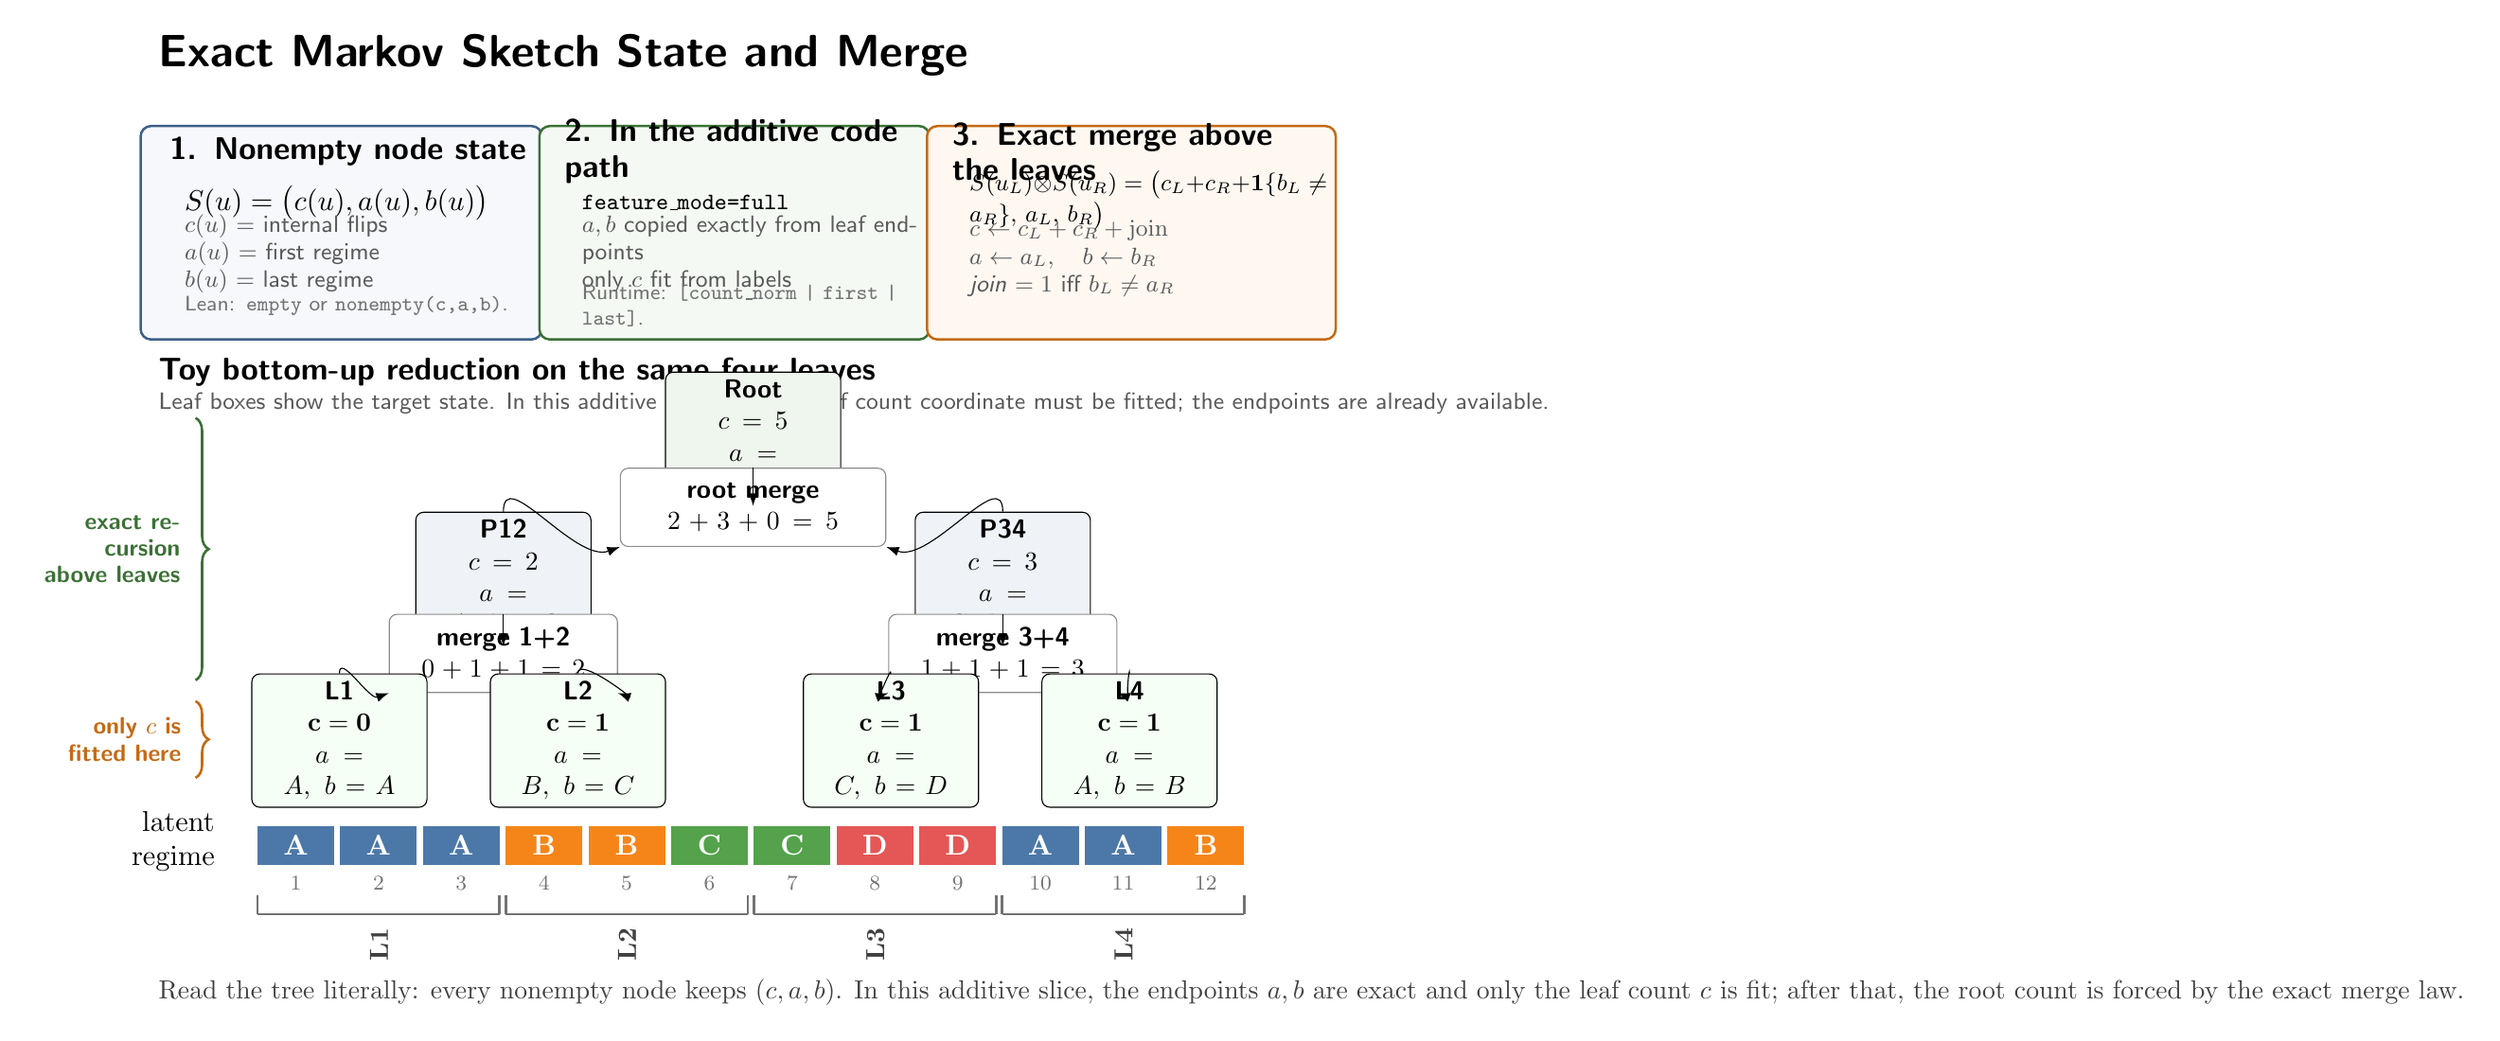
\begin{tikzpicture}[x=1cm,y=1cm,font=\sffamily,>=Latex]
  \node[anchor=west, align=left, text width=15.7cm, font=\sffamily\bfseries\fontsize{16.0}{18.0}\selectfont] at (0, 9.25)
    {Exact Markov Sketch State and Merge};

  \node[anchor=west, align=left, text width=4.85cm, font=\sffamily\bfseries\fontsize{11.8}{13.6}\selectfont] at (0.15, 7.95)
    {1. Nonempty node state};
  \node[anchor=west, font=\sffamily\fontsize{11.0}{13.0}\selectfont] at (0.35, 7.26)
    {$S(u)=\big(c(u), a(u), b(u)\big)$};
  \node[anchor=west, align=left, text width=4.65cm, text=black!65, font=\sffamily\fontsize{8.8}{10.6}\selectfont] at (0.35, 6.58)
    {$c(u)$ = internal flips\\
     $a(u)$ = first regime\\
     $b(u)$ = last regime};
  \node[anchor=west, align=left, text width=4.7cm, text=black!55, font=\sffamily\fontsize{8.2}{9.9}\selectfont] at (0.35, 5.88)
    {Lean: \texttt{empty} or \texttt{nonempty(c,a,b)}.};
  \begin{scope}[on background layer]
    \node[panel, draw=regA!80!black, fill=regA!5, fit={(0.0,5.55) (5.15,8.18)}] {};
  \end{scope}

  \node[anchor=west, align=left, text width=4.7cm, font=\sffamily\bfseries\fontsize{11.8}{13.6}\selectfont] at (5.45, 7.95)
    {2. In the additive code path};
  \node[anchor=west, align=left, text width=4.55cm, font=\sffamily\fontsize{9.1}{10.9}\selectfont] at (5.68, 7.27)
    {\textbf{\texttt{feature\_mode=full}}};
  \node[anchor=west, align=left, text width=4.55cm, text=black!65, font=\sffamily\fontsize{8.8}{10.6}\selectfont] at (5.68, 6.58)
    {$a,b$ copied exactly from leaf endpoints\\
     only $c$ fit from labels};
  \node[anchor=west, align=left, text width=4.55cm, text=black!55, font=\sffamily\fontsize{8.2}{9.9}\selectfont] at (5.68, 5.88)
    {Runtime: \texttt{[count\_norm | first | last]}.};
  \begin{scope}[on background layer]
    \node[panel, draw=regC!70!black, fill=regC!6, fit={(5.35,5.55) (10.35,8.18)}] {};
  \end{scope}

  \node[anchor=west, align=left, text width=5.0cm, font=\sffamily\bfseries\fontsize{11.8}{13.6}\selectfont] at (10.65, 7.95)
    {3. Exact merge above the leaves};
  \node[anchor=west, align=left, text width=4.8cm, font=\sffamily\fontsize{8.95}{10.75}\selectfont] at (10.88, 7.30)
    {$S(u_L)\otimes S(u_R)=\big(c_L+c_R+\mathbf{1}\{b_L\neq a_R\},\, a_L,\, b_R\big)$};
  \node[anchor=west, align=left, text width=4.8cm, text=black!65, font=\sffamily\fontsize{8.7}{10.5}\selectfont] at (10.88, 6.52)
    {$c \leftarrow c_L + c_R + \mathrm{join}$\\
     $a \leftarrow a_L,\quad b \leftarrow b_R$\\
     \textit{join} $=1$ iff $b_L \neq a_R$};
  \begin{scope}[on background layer]
    \node[panel, draw=regB!80!black, fill=regB!6, fit={(10.55,5.55) (15.8,8.18)}] {};
  \end{scope}

  \node[anchor=west, font=\sffamily\bfseries\fontsize{13.2}{15.2}\selectfont] at (0, 5.00)
    {Toy bottom-up reduction on the same four leaves};
  \node[anchor=west, text=black!65, font=\sffamily\fontsize{9.3}{11.0}\selectfont] at (0, 4.58)
    {Leaf boxes show the target state. In this additive slice, only the leaf count coordinate must be fitted; the endpoints are already available.};

  \node[sum, fill=regC!10, text width=1.95cm] (root) at (8.10, 4.10) {\textbf{Root}\\$c=5$\\$a=A,\; b=B$};
  \node[sum, draw=black!45, fill=white, text width=3.35cm] (croot) at (8.10, 3.18)
    {\textbf{root merge}\\$2 + 3 + 0 = 5$};
  \node[sum, fill=regA!9, text width=1.95cm] (m12) at (4.75, 2.22) {\textbf{P12}\\$c=2$\\$a=A,\; b=C$};
  \node[sum, fill=regA!9, text width=1.95cm] (m34) at (11.45, 2.22) {\textbf{P34}\\$c=3$\\$a=C,\; b=B$};
  \node[sum, draw=black!45, fill=white, text width=2.85cm] (c12) at (4.75, 1.22)
    {\textbf{merge 1+2}\\$0 + 1 + 1 = 2$};
  \node[sum, draw=black!45, fill=white, text width=2.85cm] (c34) at (11.45, 1.22)
    {\textbf{merge 3+4}\\$1 + 1 + 1 = 3$};
  \node[sum, fill=green!4, text width=1.95cm] (l1) at (2.55, 0.05) {\textbf{L1}\\$\mathbf{c=0}$\\$a=A,\; b=A$};
  \node[sum, fill=green!4, text width=1.95cm] (l2) at (5.75, 0.05) {\textbf{L2}\\$\mathbf{c=1}$\\$a=B,\; b=C$};
  \node[sum, fill=green!4, text width=1.95cm] (l3) at (9.95, 0.05) {\textbf{L3}\\$\mathbf{c=1}$\\$a=C,\; b=D$};
  \node[sum, fill=green!4, text width=1.95cm] (l4) at (13.15, 0.05) {\textbf{L4}\\$\mathbf{c=1}$\\$a=A,\; b=B$};

  \draw[->] (l1.north) to[out=90,in=-160] (c12.south west);
  \draw[->] (l2.north) to[out=90,in=-20] (c12.south east);
  \draw[->] (c12.north) -- (m12.south);
  \draw[->] (l3.north) to[out=90,in=-160] (c34.south west);
  \draw[->] (l4.north) to[out=90,in=-20] (c34.south east);
  \draw[->] (c34.north) -- (m34.south);
  \draw[->] (m12.north) to[out=90,in=-160] (croot.south west);
  \draw[->] (m34.north) to[out=90,in=-20] (croot.south east);
  \draw[->] (croot.north) -- (root.south);

  \draw[decorate, decoration={brace, amplitude=5pt}, line width=0.95pt, regB!80!black]
    (0.62, 0.58) -- (0.62, -0.45)
    node[midway, xshift=-1.12cm, align=right, text width=1.85cm, font=\sffamily\bfseries\fontsize{9.1}{10.2}\selectfont, text=regB!80!black]
    {only $c$ is\\ fitted here};
  \draw[decorate, decoration={brace, amplitude=5pt}, line width=0.95pt, regC!70!black]
    (0.62, 4.38) -- (0.62, 0.86)
    node[midway, xshift=-1.18cm, align=right, text width=1.95cm, font=\sffamily\bfseries\fontsize{9.1}{10.2}\selectfont, text=regC!70!black]
    {exact recursion\\ above leaves};

  \node[anchor=east, align=right, font=\fontsize{11}{13}\selectfont] at (1.0, -1.30) {latent\\regime};
  \foreach \r/\c/\x in {
    A/regA/1.45,
    A/regA/2.56,
    A/regA/3.67,
    B/regB/4.78,
    B/regB/5.89,
    C/regC/7.00,
    C/regC/8.11,
    D/regD/9.22,
    D/regD/10.33,
    A/regA/11.44,
    A/regA/12.55,
    B/regB/13.66
  }{
    \fill[\c] (\x, -1.62) rectangle ++(1.03, 0.52);
    \node[font=\bfseries\fontsize{11}{12}\selectfont, text=white] at (\x+0.515, -1.36) {\r};
  }
  \foreach \n/\x in {1/1.965,2/3.075,3/4.185,4/5.295,5/6.405,6/7.515,7/8.625,8/9.735,9/10.845,10/11.955,11/13.065,12/14.175}{
    \node[font=\fontsize{8.5}{9.5}\selectfont, text=black!55] at (\x, -1.87) {\n};
  }
  \foreach \left/\right/\mid/\lab in {
    1.45/4.70/3.08/L1,
    4.78/8.03/6.41/L2,
    8.11/11.36/9.74/L3,
    11.44/14.69/13.07/L4
  }{
    \draw[black!55, line width=1.0pt] (\left,-2.02) -- (\left,-2.28);
    \draw[black!55, line width=1.0pt] (\left,-2.28) -- (\right,-2.28);
    \draw[black!55, line width=1.0pt] (\right,-2.02) -- (\right,-2.28);
    \node[font=\bfseries\fontsize{10.2}{11.2}\selectfont, text=black!75, rotate=90] at (\mid,-2.69) {\lab};
  }

  \node[anchor=west, text=black!75, font=\fontsize{10}{12}\selectfont] at (0, -3.33)
    {Read the tree literally: every nonempty node keeps $(c,a,b)$. In this additive slice, the endpoints $a,b$ are exact and only the leaf count $c$ is fit; after that, the root count is forced by the exact merge law.};
\end{tikzpicture}

\end{document}
